\documentclass[12pt,a4paper]{article}
\usepackage[utf8]{inputenc}
\usepackage[T1]{fontenc}
\usepackage[brazilian]{babel}
\usepackage{geometry}
\geometry{top=2.5cm, bottom=2.5cm, left=2.5cm, right=2.5cm}
\usepackage{graphicx}
\usepackage{booktabs}
\usepackage{xcolor}
\usepackage{listings}
\usepackage{hyperref}
\usepackage{amsmath}
\usepackage{amssymb}
\usepackage{titlesec}
\usepackage{enumitem}
\usepackage{tikz}
\usepackage{tabularx}
\usepackage{caption}
\usepackage{underscore}

\usetikzlibrary{shapes.geometric, arrows.meta, positioning}

% Definição de Cores Corporativas/Técnicas
\definecolor{primaryColor}{RGB}{0, 51, 102}     % Azul Escuro / Visa-ish
\definecolor{secondaryColor}{RGB}{243, 114, 44} % Laranja / Mastercard-ish
\definecolor{darkGray}{RGB}{40, 40, 40}
\definecolor{lightGray}{RGB}{248, 249, 250}
\definecolor{accentBlue}{RGB}{33, 150, 243}

% Configuração do Layout e Cabeçalhos
\titleformat{\section}{\large\bfseries\color{primaryColor}}{\thesection}{1em}{}[{\titlerule[1pt]}]
\titleformat{\subsection}{\subsectionfont\bfseries\color{primaryColor!80!black}}{\thesubsection}{1em}{}
\newcommand{\subsectionfont}{\normalsize}

\setlist[description]{style=nextline, leftmargin=1em}

% Configuração do Hyperref
\hypersetup{
    colorlinks=true,
    linkcolor=primaryColor,
    filecolor=magenta,      
    urlcolor=accentBlue,
    pdftitle={Proposta Técnica: Pipeline de IA para Extração e Estruturação Automática de Taxas de Intercâmbio},
    pdfauthor={Dr. Ademir Batista dos Santos Neto}
}

% Configuração de Código Fonte (Listings)
\lstset{
    backgroundcolor=\color{lightGray},
    basicstyle=\small\ttfamily\color{darkGray},
    breakatwhitespace=false,
    breaklines=true,
    captionpos=b,
    keepspaces=true,
    numbers=left,
    numberstyle=\tiny\color{gray},
    showspaces=false,
    showstringspaces=false,
    showtabs=false,
    tabsize=2,
    frame=single,
    rulecolor=\color{primaryColor!30},
    keywordstyle=\color{primaryColor}\bfseries,
    commentstyle=\color{gray}\itshape,
    stringstyle=\color{secondaryColor},
    extendedchars=true,
    literate=
        {á}{{\'{a}}}1 {é}{{\'{e}}}1 {í}{{\'{i}}}1 {ó}{{\'{o}}}1 {ú}{{\'{u}}}1
        {Á}{{\'{A}}}1 {É}{{\'{E}}}1 {Í}{{\'{I}}}1 {Ó}{{\'{O}}}1 {Ú}{{\'{U}}}1
        {à}{{\`{a}}}1 {è}{{\`{e}}}1 {ì}{{\`{i}}}1 {ò}{{\`{o}}}1 {ù}{{\`{u}}}1
        {â}{{\^{a}}}1 {ê}{{\^{e}}}1 {î}{{\^{i}}}1 {ô}{{\^{o}}}1 {û}{{\^{u}}}1
        {ã}{{\~{a}}}1 {õ}{{\~{o}}}1 {ç}{{\c{c}}}1 {Ç}{{\c{C}}}1
        {ã}{{\~{a}}}1 {ñ}{{\~{n}}}1 {ü}{{\"u}}1 {ö}{{\"o}}1
}

\begin{document}

% --- CAPA / CABEÇALHO ---
\begin{center}
    {\large \textbf{\color{primaryColor}PROPOSTA TÉCNICA}} \\[0.3cm]
    {\Large \textbf{\color{primaryColor}Pipeline de IA para Extração e Estruturação Automática de Taxas de Intercâmbio --- Visa \& Mastercard}} \\[0.6cm]
    
    \begin{minipage}{0.9\textwidth}
        \centering
        \small
        \color{darkGray}
        \textbf{Documento de Entrega --- Desafio Técnico Bolsista Doutor Bandeiras} \\
        Versão 1.0 \quad | \quad Junho de 2026
    \end{minipage}
\end{center}

\vspace{0.5cm}
\noindent\rule{\textwidth}{1.5pt}
\vspace{0.2cm}

% --- SUMÁRIO ---
\tableofcontents
\vspace{0.8cm}
\noindent\rule{\textwidth}{0.5pt}
\vspace{0.8cm}

% --- SEÇÃO 1 ---
\section{Análise Exploratória dos Documentos}

\subsection{Estrutura Geral dos Manuais}

Os manuais de taxas de intercâmbio da Visa e Mastercard são documentos técnicos publicados periodicamente em formato PDF. Para a montagem desta proposta de pipeline, foram considerados dois documentos como base:
\begin{itemize}
    \item \textbf{Visa USA Interchange Reimbursement Fees} --- versão de 18 de abril de 2026.
    \item \textbf{Mastercard U.S. Region Interchange Programs and Rates 2025–2026} --- vigente a partir de 11 de abril de 2025.
\end{itemize}

Ambos os documentos compartilham uma arquitetura tabular densa, porém com diferenças significativas de nomenclatura, hierarquia e segmentação, conforme detalhado na Tabela~\ref{tab:caracteristicas}.

\begin{table}[htbp]
\centering
\caption{Comparativo de Características dos Manuais Visa e Mastercard}
\label{tab:caracteristicas}
\small
\begin{tabularx}{\textwidth}{l p{5.5cm} p{5.5cm}}
\toprule
\textbf{Característica} & \textbf{Visa} & \textbf{Mastercard} \\
\midrule
Nº médio de tabelas & $\sim$25--35 & $\sim$20--30 \\
Hierarquia de produto & Infinite / Signature / Traditional / Check / Prepaid & World Elite / World High Value / World / Enhanced Value / Core \\
Dimensão de segmentação & Tipo de cartão $\times$ Modalidade (CP/CNP) $\times$ MCC & Tipo de cartão $\times$ Programa (Merit I, III, Supermarket...) $\times$ MCC \\
Formato de taxa & $X.XX\% + \$Y.YY$ com caps opcionais & $X.XX\% + \$Y.YY$ com caps opcionais \\
Tiers volumétricos & Sim (Supermarket Tiers 0--III) & Sim (Merit III Tiers 1--3, Supermarket Tiers 1--3) \\
Notas de rodapé críticas & Sim ($\sim$3--8 por tabela) & Sim ($\sim$4--6 por tabela) \\
\bottomrule
\end{tabularx}
\end{table}

\subsection{Padrões Tarifários e Regras de Segmentação}

A segmentação dos intercâmbios obedece a múltiplas dimensões simultaneamente. Compreendê-las é fundamental para qualquer pipeline de extração:

\begin{description}
    \item[a) Tipo de cartão (Card Product)] Visa e Mastercard diferenciam claramente cartões de crédito, débito (regulado vs. isento) e pré-pago (regulado vs. isento). A regulação referenciada é o \textit{Durbin Amendment} (Regulation II), que limita as taxas de débito regulado em $0.05\% + \$0.21$.
    
    \item[b) Presença física vs. remoto (Card Present / Card Not Present)] Todas as tabelas distinguem transações com cartão fisicamente presente (CP) das não-presenciais (CNP), incluindo e-commerce. As taxas CNP são invariavelmente superiores, refletindo maior risco de fraude.
    
    \item[c) Merchant Category Code (MCC)] O MCC é o vetor de segmentação mais granular. Exemplos de categorias com tratamento especial:
    \begin{itemize}
        \item \textbf{Supermarket} (MCC 5411): Visa pratica taxas diferenciadas por tiers de volume (Tier 0 a III), com variação de $1.18\% + \$0.05$ a $2.00\% + \$0.07$ para crédito. Mastercard segmenta similarmente com Base + Tier 1/2/3.
        \item \textbf{Petroleum/AFD} (\textit{Automated Fuel Dispenser} --- MCCs 5541, 5542): ambas as bandeiras aplicam cap de $\$0.95$, independente do percentual calculado.
        \item \textbf{Utilities} (MCCs 4900–4999): Mastercard aplica taxa fixa de $\$0.75$ por transação, sem componente percentual.
        \item \textbf{Government / Public Sector}: taxas reduzidas com caps explícitos ($\$2.00$ na Visa; segmento \textit{Public Sector} na Mastercard com $1.55\% + \$0.10$).
        \item \textbf{Charities}: ambas praticam taxas preferenciais ($2.00\% + \$0.10$ na Mastercard, independente do tier de produto).
        \item \textbf{Gaming MCCs} (Mastercard: 7800, 7801, 7802, 7994, 7995): taxa de $0.00\% + \$0.10$, refletindo tratamento de "\textit{payment transaction}".
    \end{itemize}
    
    \item[d) Modalidades especiais de transação] Conforme resumido na Tabela~\ref{tab:modalidades}.
\end{description}

\begin{table}[htbp]
\centering
\caption{Modalidades Especiais de Transação e Padrões de Taxas}
\label{tab:modalidades}
\small
\begin{tabularx}{\textwidth}{l p{5.5cm} p{5.5cm}}
\toprule
\textbf{Modalidade} & \textbf{Visa} & \textbf{Mastercard} \\
\midrule
Small Ticket ($\le \$10-\$15$) & Taxa específica, ex: $1.55\% + \$0.04$ débito & Taxa específica, ex: $1.65\% + \$0.02$ crédito CP \\
Contactless & Subsumir nas taxas CP padrão; sem linha separada & Idem \\
Pré-pago isento & Tabela B dedicada ($1.15\% + \$0.15$ base) & Coluna Prepaid Rate na tabela Debit/Prepaid \\
Key-Entered / CNP sem aut. & Taxas majoradas ($1.65\% + \$0.15$ débito) & $1.95\% + \$0.10$ crédito \\
Full UCAF (e-commerce aut.) & Taxas preferentes vs. Standard CNP & $1.95\% + \$0.10$ (crédito Core) \\
Debt Repayment & Taxa com caps distintos ($\$2.00$ e $\$0.65$) & N/A como linha separada \\
\bottomrule
\end{tabularx}
\end{table}

\subsection{Desafios na Leitura dos PDFs}

\begin{description}
    \item[Desafio 1 --- Tabelas multi-header hierárquicas.] As tabelas da Visa possuem até três níveis de cabeçalho: (i) seção do documento (ex: ``Consumer Credit''), (ii) modalidade (Card Present / Card Not Present), e (iii) produto (Visa Infinite / Signature...). O parser deve resolver essa hierarquia para associar cada célula a seus eixos corretos.
    
    \item[Desafio 2 --- Notas de rodapé como modificadores de regra.] Asteriscos, superescritos numéricos e letras referenciam condições que alteram o valor principal. Por exemplo, na Visa: \texttt{*} indica adicional de $\$0.01$ para issuers com certificação de prevenção de fraude; \texttt{1} restringe a taxa de Small Ticket a transações na rede 002. Ignorar estas notas produz dados incorretos para casos de uso reais.
    
    \item[Desafio 3 --- Caps e valores mínimos embutidos em células.] A formatação $1.90\% + \$0.00 \text{ (0.95 max)}$ da Mastercard Petroleum e $0.80\% + \$0.15 \text{ (\$0.15 min / \$2.00 max)}$ da Visa exige parsing de estrutura interna da célula, não apenas extração de texto.
    
    \item[Desafio 4 --- Tiers volumétricos com critérios de qualificação em tabelas auxiliares.] Os critérios de elegibilidade aos tiers (ex: Mastercard Merit III Tier 1 exige volume mínimo anual de USD 1,80 bilhão) aparecem em tabelas separadas dos valores das taxas. O pipeline precisa juntar estas entidades.
    
    \item[Desafio 5 --- Variação de layout entre versões.] As bandeiras alteram layout, nomenclatura e ordem das tabelas entre publicações semestrais. Um pipeline robusto não pode depender de posições fixas de células.
    
    \item[Desafio 6 --- Conteúdo misto (texto narrativo + tabelas).] Parágrafos introdutórios e notas legais intercalam-se com as tabelas. O pipeline deve distinguir blocos de prosa dos blocos tabulares.
\end{description}

\newpage

% --- SEÇÃO 2 ---
\section{Proposta de Pipeline para Extração e Estruturação}

A arquitetura proposta é inspirada no framework \textbf{RAG (Retrieval-Augmented Generation)} e organizada em cinco estágios principais: \textbf{Ingestion $\rightarrow$ Chunking $\rightarrow$ Embedding $\rightarrow$ Indexing $\rightarrow$ Retrieval + LLM}.

\subsection{Visão Geral do Fluxo}

\begin{figure}[htbp]
\centering
\small
\begin{tikzpicture}[
    node distance=1.5cm,
    block/.style={rectangle, draw=primaryColor, fill=lightGray, thick, minimum width=4cm, minimum height=0.8cm, align=center, rounded corners=2pt},
    line/.style={draw=primaryColor, thick, -{Stealth[scale=1.2]}}
]
    % Nos do Pipeline
    \node (pdf) [block] { [PDF Bandeira] };
    \node (ocr) [block, below=of pdf] { Ingestão \& OCR };
    \node (chunk) [block, below=of ocr] { Chunking Estrutural };
    \node (llm) [block, below=of chunk] { Extração Semântica via LLM };
    \node (val) [block, below=of llm] { Validação \& Reconciliação };
    \node (db) [block, below=of val] { Banco de Dados Estruturado };
    
    % Ramos Laterais
    \node (embed) [block, left=2cm of db] { Embedding };
    \node (vector) [block, above=of embed] { Vector Store para RAG };
    \node (agent) [block, right=2cm of db] { Agente de Consulta \\ / Dashboard };

    % Conexões
    \path [line] (pdf) -- (ocr);
    \path [line] (ocr) -- (chunk);
    \path [line] (chunk) -- (llm);
    \path [line] (llm) -- (val);
    \path [line] (val) -- (db);
    \path [line] (db) -- (embed);
    \path [line] (embed) -- (vector);
    \path [line] (db) -- (agent);
\end{tikzpicture}
\caption{Diagrama de Blocos da Arquitetura do Pipeline}
\label{fig:pipeline_flow}
\end{figure}

\subsection{Estágio 1 --- Ingestão do PDF}

\textbf{Objetivo:} Converter o PDF em representações intermediárias que preservem a estrutura (tabelas, hierarquia de cabeçalhos, notas de rodapé).

\begin{table}[htbp]
\centering
\caption{Ferramentas Recomendadas para Ingestão}
\small
\begin{tabularx}{\textwidth}{l p{4cm} p{7cm}}
\toprule
\textbf{Ferramenta} & \textbf{Papel} & \textbf{Justificativa} \\
\midrule
\texttt{pdfplumber} & Extração de tabelas com bounding boxes & Preserva posição de células; lida com tabelas sem bordas explícitas \\
\texttt{pymupdf} (fitz) & Extração de texto bruto e blocos & Alta performance; suporte a metadados de página \\
\texttt{unstructured} & Classificação de elementos & Reduz trabalho de heurística manual \\
\texttt{pytesseract} & OCR de fallback & Suporte para páginas escaneadas ou artefatos \\
\texttt{camelot} & Extração alternativa de tabelas & Robusto para formatos tipo lattice/stream \\
\bottomrule
\end{tabularx}
\end{table}

\textbf{Processo detalhado:}
\begin{enumerate}
    \item Abertura do PDF via \texttt{pdfplumber}; iteração por página.
    \item Detecção de blocos tabulares via bounding boxes.
    \item Extração de texto narrativo separadamente (introduções, notas legais).
    \item Aplicação de OCR seletivo em páginas onde a extração digital falha.
    \item Saída: lista de objetos \texttt{PageBlock} com tipo (\texttt{table} | \texttt{text} | \texttt{footnote}), conteúdo bruto e coordenadas.
\end{enumerate}

\begin{figure}[htbp]
\centering
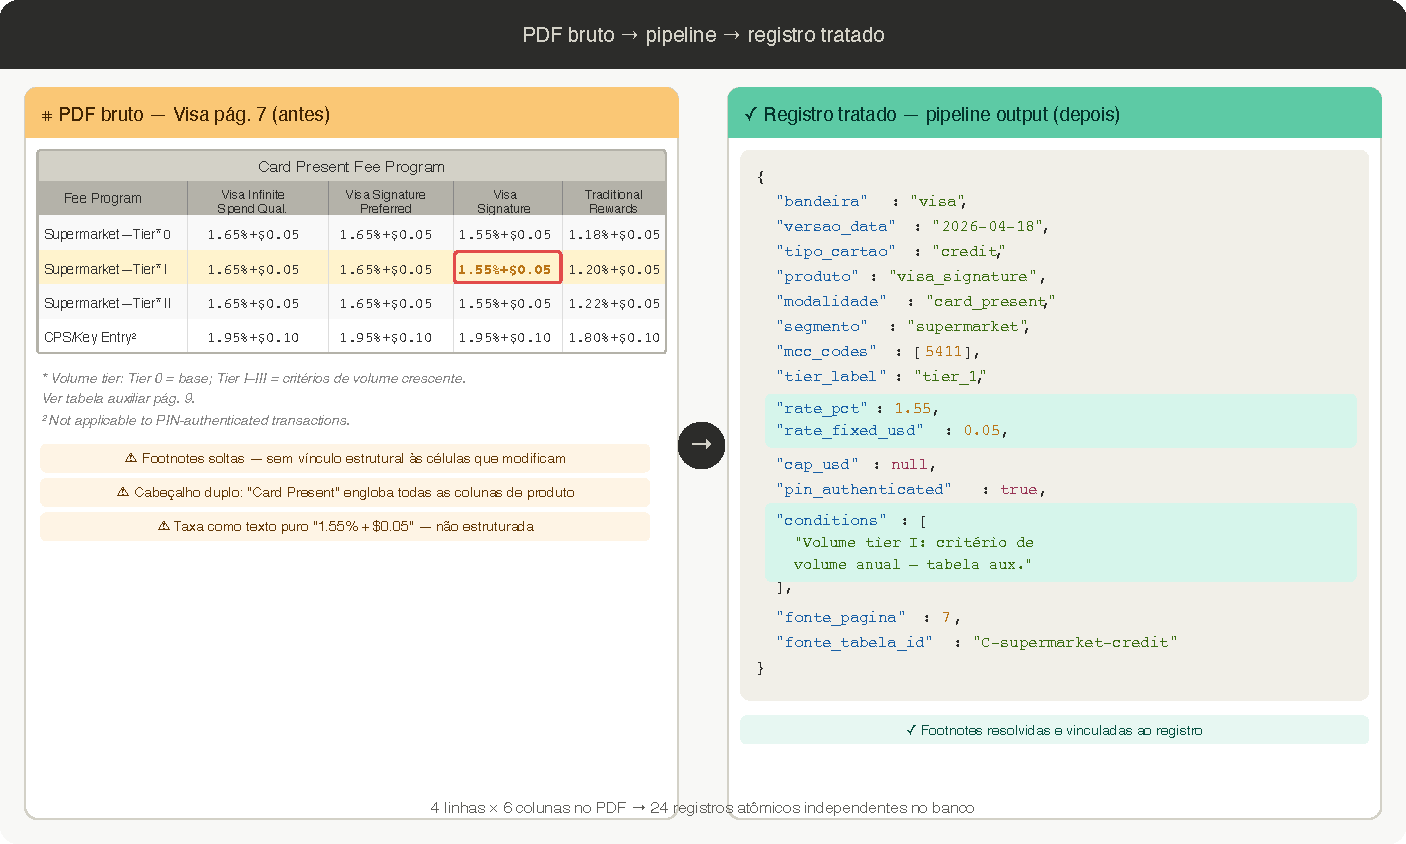
\includegraphics[width=\textwidth]{comparativo_pipeline.pdf}
\caption{Representação Conceitual do Comparativo de Processamento do Pipeline}
\label{fig:comparativo_pipeline}
\end{figure}

\subsection{Estágio 2 --- Chunking Estrutural}

\textbf{Objetivo:} Dividir o conteúdo em unidades semânticas coerentes, preservando contexto hierárquico. Esta etapa diverge do chunking tradicional por tokens porque o domínio exige \textbf{chunking orientado a entidade de regra}.

\begin{center}
\small
\begin{minipage}{0.85\textwidth}
\textbf{Estratégia de chunking em três camadas:}
\begin{itemize}[label=$\rightarrow$]
    \item \textbf{Nível 1:} Seção do documento
    \begin{itemize}[label=$\rightarrow$]
        \item \textbf{Nível 2:} Tabela (com todos os seus cabeçalhos resolvidos)
        \begin{itemize}[label=$\rightarrow$]
            \item \textbf{Nível 3:} Linha de regra (combinação MCC $\times$ Produto $\times$ Modalidade $\times$ Taxa)
        \end{itemize}
    \end{itemize}
\end{itemize}
\end{minipage}
\end{center}

Cada \textbf{chunk de Nível 3} é a unidade mínima indexável e deve conter contextos herdados dos níveis superiores, valores de taxa, referências resolvidas a notas de rodapé e metadados estruturais (\texttt{page_number}, \texttt{table_id}, \texttt{version_date}).

\begin{lstlisting}[language=Python, caption=Pseudocódigo de resolução de multi-header]
def resolve_headers(raw_table: list[list[str]]) -> list[dict]:
    header_rows = detect_header_rows(raw_table)  
    merged_header = merge_hierarchical_headers(header_rows)
    data_rows = raw_table[len(header_rows):]
    return [
        {col: row[i] for i, col in enumerate(merged_header)}
        for row in data_rows
    ]
\end{lstlisting}

\textbf{Resolução de notas de rodapé:} As notas são extraídas como entidades separadas e vinculadas aos chunks por referência de símbolo (\texttt{*}, \texttt{1}, \texttt{a}). Um LLM local via Ollama (\texttt{llama3.2} ou \texttt{qwen2.5:3b}) é usado para parafrasear a nota em linguagem estruturada.

\subsection{Estágio 3 --- Embedding e Indexação}

\textbf{Objetivo:} Converter chunks em vetores densos para busca semântica pelo Agente de Consulta. Recomendam-se os modelos \texttt{text-embedding-3-large} (OpenAI) ou \texttt{BAAI/bge-m3}.

\begin{table}[htbp]
\centering
\caption{Estratégias de Indexação de Vetores}
\small
\begin{tabularx}{\textwidth}{l p{4.5cm} p{6.5cm}}
\toprule
\textbf{Estratégia} & \textbf{Quando usar} & \textbf{Configuração} \\
\midrule
\textbf{HNSW} & Operação interativa (Q\&A em tempo real) & Latência $<$ 10ms; dataset $<$ 10M vetores \\
\textbf{IVF} & Batch analytics, re-processamento & Corpus estável; controle de memória de hardware \\
\bottomrule
\end{tabularx}
\end{table}

\textbf{Vector Store recomendado:} \textbf{Qdrant} ou \textbf{Weaviate} (suporte nativo a payload filtering e hybrid search).

\begin{lstlisting}[language={}, caption=Exemplo de Payload de Metadados Indexados]
{
  "bandeira": "visa",
  "tipo_cartao": "credit",
  "produto": "visa_signature",
  "modalidade": "card_not_present",
  "segmento": "supermarket",
  "mcc_range": "5411",
  "version_date": "2026-04-18",
  "regulated": false
}
\end{lstlisting}

\subsection{Estágio 4 --- Extração Semântica via LLM/Agente}

\textbf{Objetivo:} Usar um LLM como leitor inteligente para resolver ambiguidades e converter tabelas brutas em registros JSON normalizados.

\begin{figure}[htbp]
\centering
\small
\begin{tikzpicture}[
    node box/.style={rectangle, draw=primaryColor, fill=lightGray, thick, minimum width=8cm, minimum height=3.5cm, align=left, rounded corners=4pt}
]
    \node (agent) [node box] {
        \textbf{\color{primaryColor}AGENTE DE EXTRAÇÃO (LLM)} \\[0.2cm]
        \texttt{Tool 1: parse_table_chunk(raw_html_table)} \\
        \texttt{Tool 2: resolve_footnote(symbol, footnote_text)} \\
        \texttt{Tool 3: validate_rate_format(rate_string)} \\
        \texttt{Tool 4: classify_mcc(description)} \\
        \texttt{Tool 5: detect_cap_or_floor(cell_text)}
    };
\end{tikzpicture}
\caption{Arquitetura e Ferramentas do Agente de Extração}
\label{fig:agente_tools}
\end{figure}

Para a extração de tabelas financeiras densas, recomenda-se o uso de modelos estruturados nativos de alta capacidade como \texttt{llama3.1:70b} ou \texttt{qwen2.5:72b} para evitar alucinações.

\subsection{Estágio 5 --- Validação e Reconciliação}

\begin{enumerate}
    \item \textbf{Validação de formato:} Garantir que \texttt{rate_pct} $\in [0, 5]$, \texttt{rate_fixed} $\in [0, 2]$ e caps sejam positivos.
    \item \textbf{Validação de completude:} Disparar alertas caso campos obrigatórios estejam ausentes.
    \item \textbf{Validação cruzada:} Verificar consistência histórica de programas equivalentes.
    \item \textbf{Validação por versão:} Identificar variações bruscas ($> 0.5\text{pp}$) comparativamente à versão anterior.
\end{enumerate}
\textbf{Framework:} Uso do \texttt{Great Expectations} (Python) com alertas via webhook.

\newpage

% --- SEÇÃO 3 ---
\section{Abordagem Técnica e Modelagem de Banco de Dados}

\subsection{Arquitetura Híbrida: Relacional + Vetorial}
Propõe-se o uso do \textbf{PostgreSQL} (com extensão \texttt{TimescaleDB}) para queries determinísticas e simulações analíticas, operando em paralelo ao \textbf{Qdrant} para recuperação semântica do Agente RAG.

\begin{figure}[htbp]
\centering
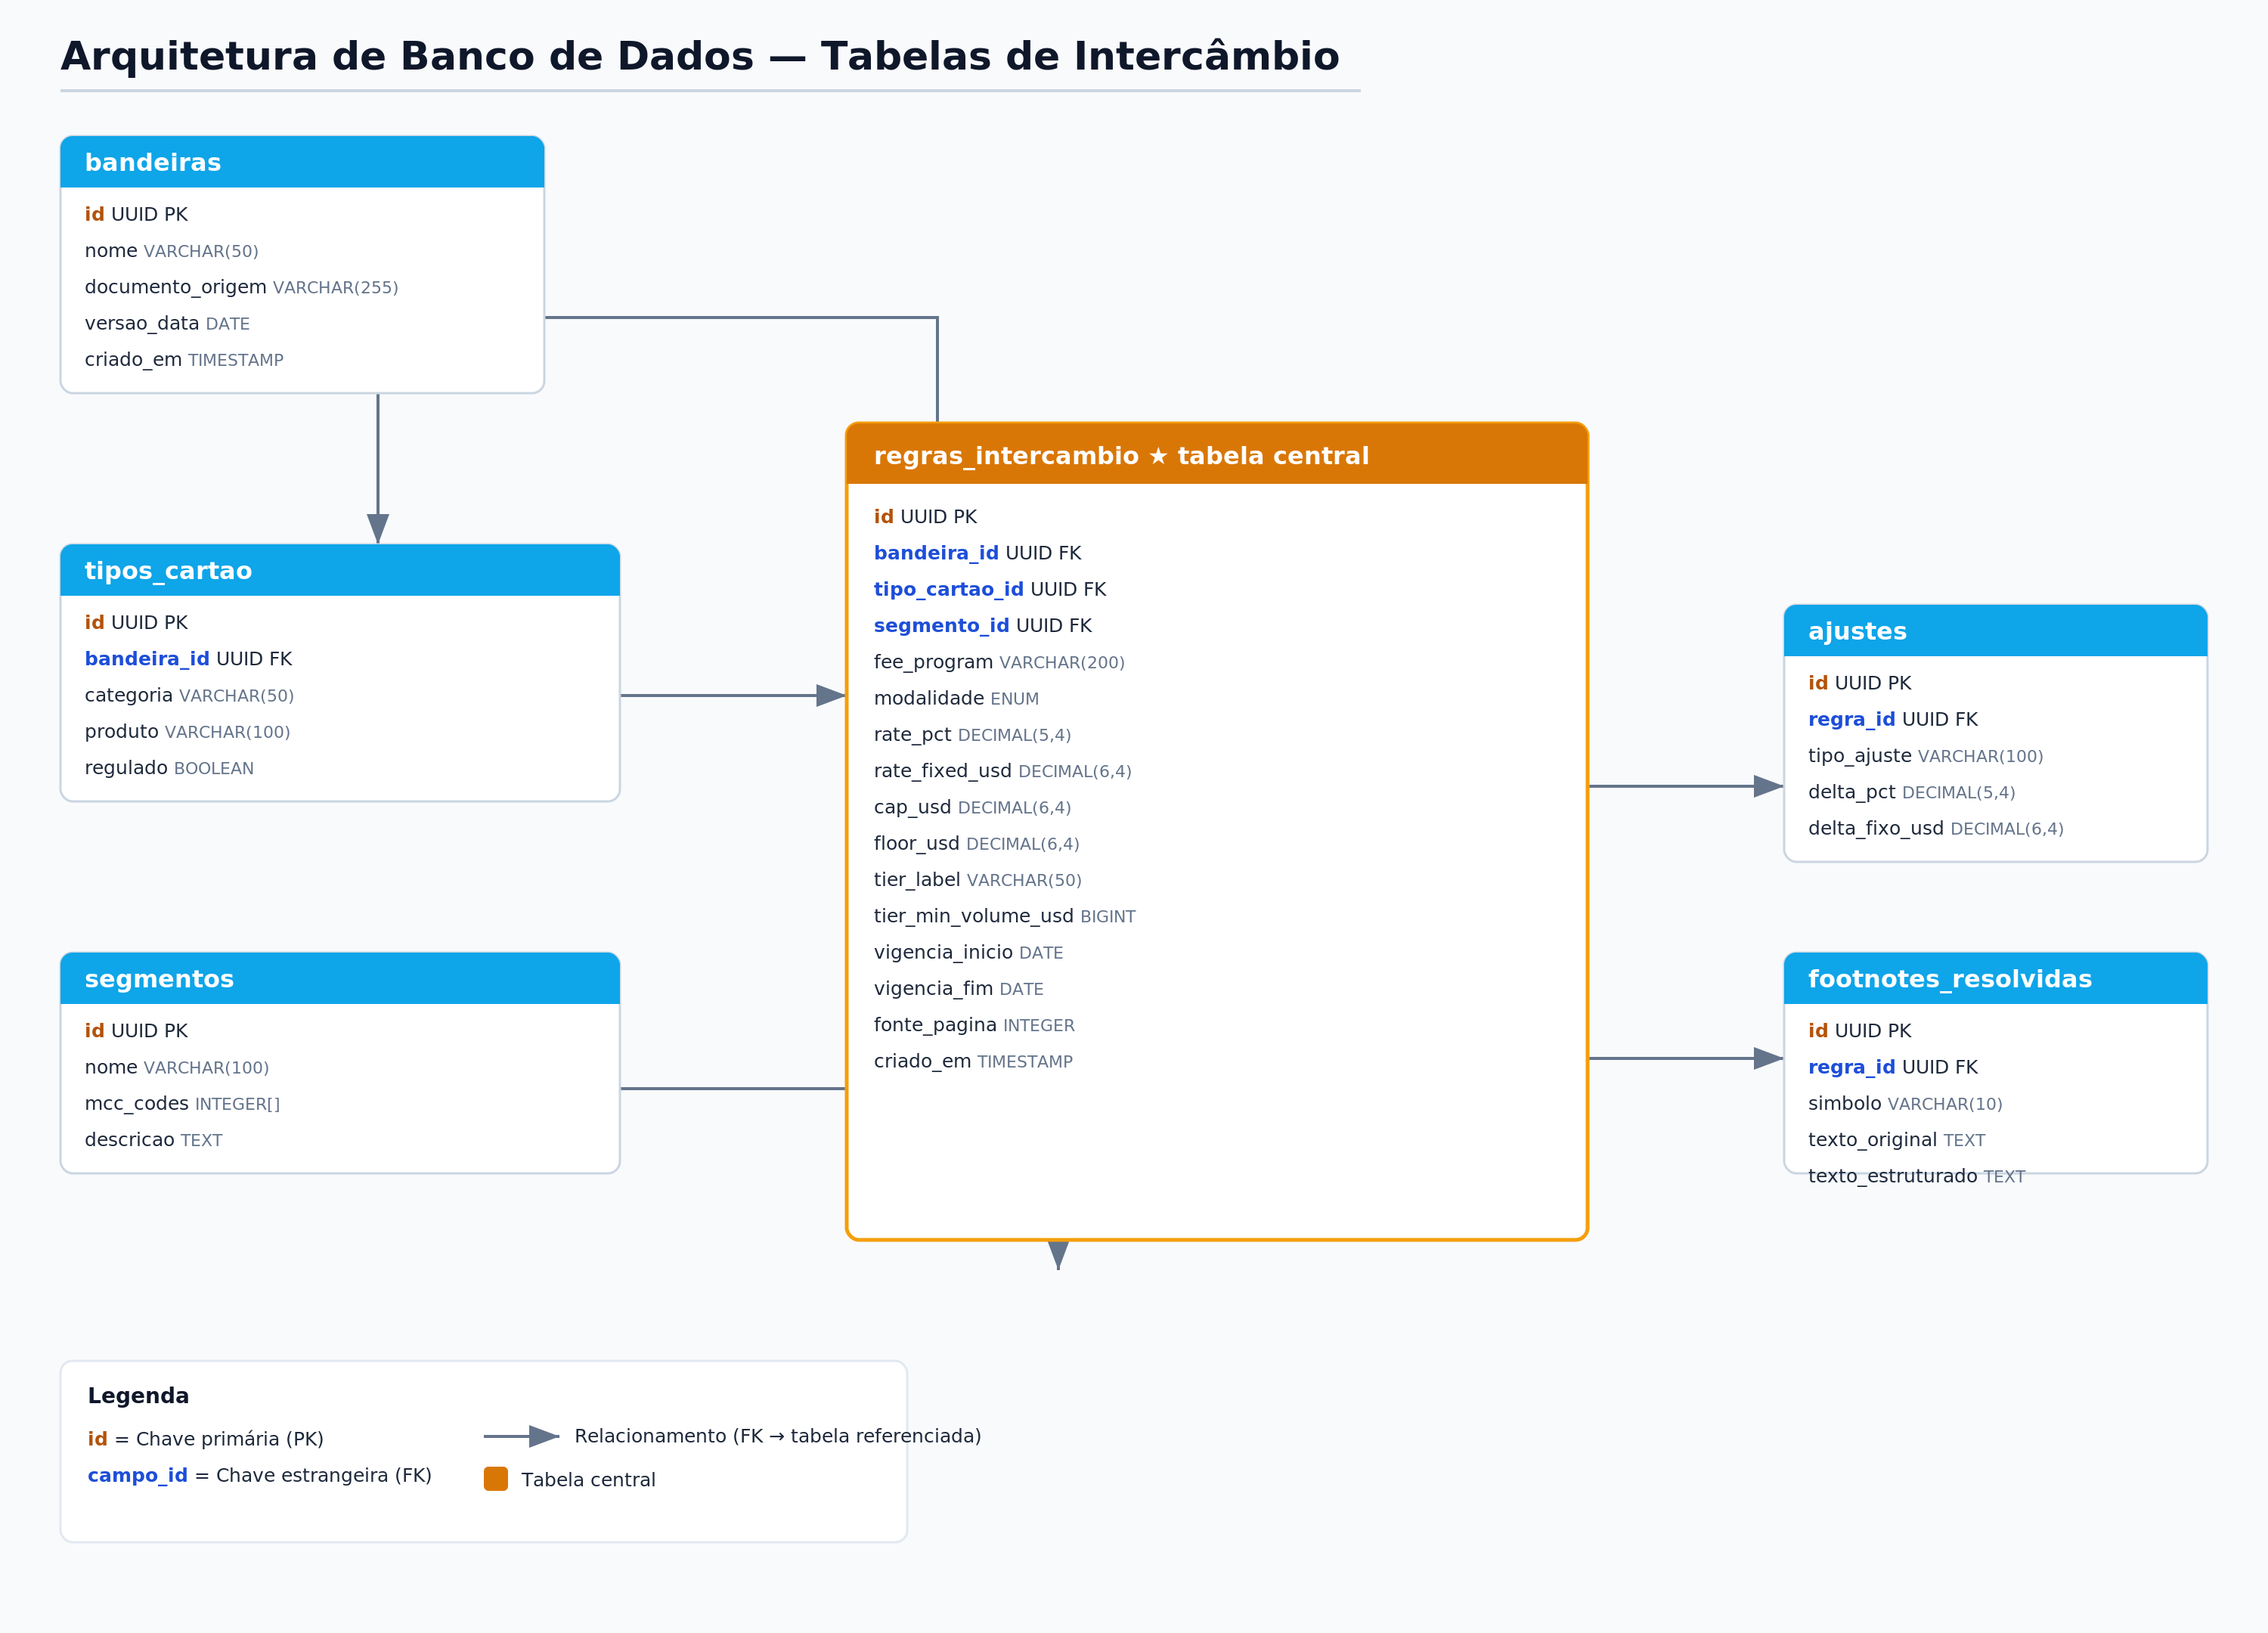
\includegraphics[width=\textwidth]{arquitetura_db.png}
\caption{Arquitetura Híbrida: Banco Relacional (PostgreSQL) e Vetorial (Qdrant)}
\label{fig:arquitetura_db}
\end{figure}

\subsection{Esquema Relacional (DDL Simplificado)}

Abaixo são apresentadas as estruturas das tabelas principais da camada relacional.

\subsubsection{Tabela \texttt{bandeiras}}
\begin{tabularx}{\textwidth}{llX}
\toprule
\textbf{Campo} & \textbf{Tipo} & \textbf{Descrição} \\
\midrule
\texttt{id} & UUID PK & Identificador único da bandeira \\
\texttt{nome} & VARCHAR(50) & Ex: ``visa'', ``mastercard'' \\
\texttt{documento\_origem} & VARCHAR(255) & Caminho ou hash do PDF fonte \\
\texttt{versao\_data} & DATE & Data de vigência das taxas \\
\bottomrule
\end{tabularx}

\subsubsection{Tabela \texttt{regras\_intercambio} (Tabela Central)}
\begin{tabularx}{\textwidth}{llX}
\toprule
\textbf{Campo} & \textbf{Tipo} & \textbf{Descrição} \\
\midrule
\texttt{id} & UUID PK & Identificador único da regra \\
\texttt{bandeira\_id} & UUID FK & Relacionamento com tabela \texttt{bandeiras} \\
\texttt{fee\_program} & VARCHAR(200) & Nome original do programa (ex: ``CPS/Retail'') \\
\texttt{modalidade} & ENUM & \texttt{card\_present} ou \texttt{card\_not\_present} \\
\texttt{rate\_pct} & DECIMAL(5,4) & Percentual da taxa (ex: 0.0165 para 1.65\%) \\
\texttt{rate\_fixed\_usd} & DECIMAL(6,4) & Componente fixo em dólar (ex: 0.15) \\
\texttt{cap\_usd} & DECIMAL(6,4) & Valor de teto máximo (NULL se inexistente) \\
\texttt{floor\_usd} & DECIMAL(6,4) & Valor de piso mínimo (NULL se inexistente) \\
\texttt{vigencia\_inicio} & DATE & Data de início da vigência \\
\texttt{vigencia\_fim} & DATE & Data de término (NULL se atual) \\
\bottomrule
\end{tabularx}

\subsection{Consultas Analíticas Ilustrativas}

\begin{lstlisting}[language=SQL, caption=Queries de Agregação e Auditoria Analítica]
-- 1. Taxa média ponderada para e-commerce, crédito, por bandeira
SELECT 
    b.nome AS bandeira,
    AVG(r.rate_pct * 100) AS taxa_pct_media,
    AVG(r.rate_fixed_usd) AS fixo_medio_usd
FROM regras_intercambio r
JOIN bandeiras b ON r.bandeira_id = b.id
JOIN tipos_cartao tc ON r.tipo_cartao_id = tc.id
WHERE r.modalidade = 'card_not_present'
  AND tc.categoria = 'credit'
  AND r.vigencia_fim IS NULL
GROUP BY b.nome;

-- 2. Identificar programas com cap ativo por segmento
SELECT fee_program, rate_pct * 100 AS pct, rate_fixed_usd, cap_usd
FROM regras_intercambio
WHERE cap_usd IS NOT NULL
ORDER BY segmento_id, bandeira_id;
\end{lstlisting}

\newpage

% --- SEÇÃO 4 ---
\section{Visualizações Estratégicas e Dashboards}

Os dados estruturados alimentam visualizações integradas via \textbf{Metabase} conectado ao PostgreSQL.

\subsection{Visão Comparativa 1 --- Visa vs. Mastercard em E-Commerce}
Consiste em um \textbf{Heatmap de taxa efetiva} calculada sobre um ticket médio de referência de $\$50$ ($Rate\% + \frac{Fixed}{Ticket}$).

\begin{table}[htbp]
\centering
\caption{Exemplo de Matriz de Comparabilidade de Taxas Efetivas (CNP Crédito)}
\label{tab:heatmap_mock}
\small
\begin{tabularx}{\textwidth}{l X X l}
\toprule
\textbf{Segmento} & \textbf{Visa Infinite CNP} & \textbf{MC World Elite CNP} & \textbf{$\Delta$ (pp)} \\
\midrule
Supermarket & $2.00\% + \$0.07$ & $2.10\% + \$0.10$ & $\sim +0.13$ \\
Restaurant & --- & $2.00\% + \$0.10$ & --- \\
Petroleum (cap $\$0.95$) & $1.80\% + \$0.07$ & $2.00\% + \$0.00$ & Variável \\
Utilities & $\sim 1.65\% + \$0.15$ & $\$0.75$ fixo & Variável \\
Government & $0.65\% + \$0.15 \text{ (cap } \$2.00)$ & $1.55\% + \$0.10$ & Variável \\
\bottomrule
\end{tabularx}
\end{table}

\subsection{Visão Comparativa 2 --- Detalhamento por MCC e Filtros Dinâmicos}
Gráficos de barras agrupados no dashboard permitem a filtragem rápida por tipo de cartão, modalidade (CP/CNP) e tiers de produtos. KPIs centrais destacam volumetria de programas modificados e dão acesso a um \textbf{Simulador de Custo Transacional} parametrizável.

% --- SEÇÃO 5 ---
\section{Recomendações Técnicas para Evolução do Agente de IA}

\subsection{Escalabilidade e Processamento em Escala}
\begin{itemize}
    \item \textbf{Apache Airflow:} Utilizado para automação e orquestração de DAGs de ingestão baseadas no hash dos arquivos dos manuais.
    \item \textbf{Polars:} Substituição do Pandas por manipulação via \texttt{Polars}/\texttt{PyArrow} para otimização de memória em processamento batch.
\end{itemize}

\begin{lstlisting}[language=Python, caption=Normalização de Estruturas com Polars]
import polars as pl

df = pl.read_ndjson("extracted_rules.ndjson")
df_normalized = (
    df
    .with_columns([
        (pl.col("rate_pct") / 100).alias("rate_pct_decimal"),
        pl.col("cap_usd").fill_null(float("inf")).alias("cap_usd_safe"),
    ])
    .filter(pl.col("rate_pct") > 0)
    .sort(["bandeira", "tipo_cartao", "fee_program"])
)
\end{lstlisting}

\subsection{Monitoramento de Concept Drift}
Para prevenir falhas operacionais decorrentes de alterações semestrais nos layouts dos PDFs, recomenda-se a implementação de um \textbf{Hash estrutural de tabelas} (identificação de quebras de esquemas) associado à análise de \textbf{Embedding Drift} via métrica de distância de cosseno aplicável aos vetores gerados das novas tabelas.

\subsection{Mecanismos de Atenção, Re-Ranking e Segurança}
\begin{itemize}
    \item \textbf{Cross-Encoder Re-Ranking:} Aplicação do modelo \texttt{cross-encoder/ms-marco-MiniLM-L-6-v2} pós-recuperação vetorial para mitigar falsos positivos semânticos.
    \item \textbf{Filtros Temporais Restritivos:} Inclusão mandatória de metadados de vigência (\texttt{vigencia_fim IS NULL}) nas queries de busca do pipeline RAG.
    \item \textbf{Segurança e Governança:} Controle de acessos via \textit{Metadata Filtering} (estratégia \textit{Shared Index}) garantindo isolamento corporativo (\textit{multi-tenancy}) e trilhas completas de auditoria de dados.
\end{itemize}

\vspace{0.8cm}
\noindent\rule{\textwidth}{0.5pt}
\vspace{0.5cm}

\begin{flushright}
    \small
    \textbf{Dr. Ademir Batista dos Santos Neto} \\
    \textit{Cientista de Dados Sênior} \\
    Junho de 2026
\end{flushright}

\end{document}
